% mnras_template.tex 
%
% LaTeX template for creating an MNRAS paper
%
% v3.0 released 14 May 2015
% (version numbers match those of mnras.cls)
%
% Copyright (C) Royal Astronomical Society 2015
% Authors:
% Keith T. Smith (Royal Astronomical Society)

% Change log
%
% v3.0 May 2015
%    Renamed to match the new package name
%    Version number matches mnras.cls
%    A few minor tweaks to wording
% v1.0 September 2013
%    Beta testing only - never publicly released
%    First version: a simple (ish) template for creating an MNRAS paper

%%%%%%%%%%%%%%%%%%%%%%%%%%%%%%%%%%%%%%%%%%%%%%%%%%
% Basic setup. Most papers should leave these options alone.
\documentclass[fleqn,usenatbib, onecolumn,dvipdfmx]{mnras}
\usepackage{pdfpages}
\usepackage{mediabb}
% MNRAS is set in Times font. If you don't have this installed (most LaTeX
% installations will be fine) or prefer the old Computer Modern fonts, comment
% out the following line
\usepackage{newtxtext,newtxmath}
% Depending on your LaTeX fonts installation, you might get better results with one of these:
%\usepackage{mathptmx}
%\usepackage{txfonts}

% Use vector fonts, so it zooms properly in on-screen viewing software
% Don't change these lines unless you know what you are doing
\usepackage[T1]{fontenc}

% Allow "Thomas van Noord" and "Simon de Laguarde" and alike to be sorted by "N" and "L" etc. in the bibliography.
% Write the name in the bibliography as "\VAN{Noord}{Van}{van} Noord, Thomas"
\DeclareRobustCommand{\VAN}[3]{#2}
\let\VANthebibliography\thebibliography
\def\thebibliography{\DeclareRobustCommand{\VAN}[3]{##3}\VANthebibliography}


%%%%% AUTHORS - PLACE YOUR OWN PACKAGES HERE %%%%%

% Only include extra packages if you really need them. Common packages are:
\usepackage{graphicx}	% Including figure files
\usepackage{amsmath}	% Advanced maths commands
% \usepackage{amssymb}	% Extra maths symbols

%%%%%%%%%%%%%%%%%%%%%%%%%%%%%%%%%%%%%%%%%%%%%%%%%%

%%%%% AUTHORS - PLACE YOUR OWN COMMANDS HERE %%%%%

% Please keep new commands to a minimum, and use \newcommand not \def to avoid
% overwriting existing commands. Example:
%\newcommand{\pcm}{\,cm$^{-2}$}	% per cm-squared

%%%%%%%%%%%%%%%%%%%%%%%%%%%%%%%%%%%%%%%%%%%%%%%%%%

%%%%%%%%%%%%%%%%%%% TITLE PAGE %%%%%%%%%%%%%%%%%%%

% Title of the paper, and the short title which is used in the headers.
% Keep the title short and informative.
\title{Search for exoplanetary rings using TESS data}

% The list of authors, and the short list which is used in the headers.
% If you need two or more lines of authors, add an extra line using \newauthor
\author[T. Umetani et al.]{
T. Umetani,$^{1}$\thanks{E-mail: umetani-tsubasa@ed.tmu.ac.jp}
M. Aizawa,$^{2}$
Y. Ishisaki$^{1}$
\\
% List of institutions
$^{1}$Tokyo Metropolitan Unniversity, 1-1 Minami-Osawa, Hachioji-shi, Tokyo 192-0397, Japan\\
$^{2}$Shanghai Jiao Tong University, No.800, Dongchuan Road, Minhang District, Shanghai, China\\
}

% These dates will be filled out by the publisher
\date{Accepted XXX. Received YYY; in original form ZZZ}

% Enter the current year, for the copyright statements etc.
\pubyear{2022}

% Don't change these lines
\begin{document}
\label{firstpage}
\pagerange{\pageref{firstpage}--\pageref{lastpage}}
\maketitle

% Abstract of the paper
\begin{abstract}

\end{abstract}

% Select between one and six entries from the list of approved keywords.
% Don't make up new ones.
\begin{keywords}
planets and satellites: rings -- methods: data analysis -- planets and satellites: physical evolution
\end{keywords}

%%%%%%%%%%%%%%%%%%%%%%%%%%%%%%%%%%%%%%%%%%%%%%%%%%

%%%%%%%%%%%%%%%%% BODY OF PAPER %%%%%%%%%%%%%%%%%%

\section{Introduction}

\section{transit model and detection method}
\subsection{transit model with/without ring} \label{transit model with/without ring}
We used the quadratic limb darkening transit model without a planetary ring developed by Mandel \& Agol (2002) and implemented in `\texttt{batman}` (Kreidberg 2015). This model has nine parameters; $t_0, p_{\rm{orb}}, r_{\rm{p}}/r_{\rm{s}}, a/r_{\rm{s}}, b, ecc, w, q_1, q_2$. $t_0$ is the phase shift from mid-transit time, $t_{\rm{mid}}$, $p_{\rm{orb}}$ is the orbital period of the planet, $r_{\rm{p}}/r_{\rm{s}}$ is the ratio of the planet radius to the stellar radius, $a/r_{\rm{s}}$ is the orbit length radius normalized by the stellar radius, $b$ is the impact parameter, $ecc$ is the planet's eccentricity, $w$ is the longitude of the periastron and $q_{1}$ and $q_{2}$ is the limb-darkening parameters.

For the transit model with a ring, we used Aizawa et al.'s (2017) model. We assuming a single ring with uniform optical depth $\tau$ and inner radius $r_{\rm{in}}$ and outer radius $r_{\rm{out}}$. Our ringed transit model had 12 parameters: $q_1, q_2, t_0, p_{\rm{orb}}, r_{\rm{p}}/r_{\rm{s}}, a/r_{\rm{s}}, b, \theta, \phi, \tau, r_{\rm{in}}, r_{\rm{out}}$. The angle $\theta$ represents the angle between the orbital plane of the planet and the plane of the planet's ring, while $\phi$ represents the azimuthal angle. In the model fitting, we assumed an optically thick ring with $\tau=1$, and transformed $r_{\rm{in}}$ and $r_{\rm{out}}$ into dimensionless parameters using $r_{\mathrm{p}}$ as in the following 
\begin{equation}
r_{\text {in } / \mathrm{p}} \equiv \frac{r_{\text {in }}}{r_{\mathrm{p}}}, \quad r_{\mathrm{out} / \mathrm{in}} \equiv \frac{r_{\mathrm{out}}}{r_{\text {in }}}
\end{equation}

The stellar intensity profile, $I_s(x, y)$, is expressed by the following equation.

\begin{equation} \label{eq:stellar intensity}
I_s(x, y) \propto\left[1-2 q_{2} \sqrt{q_{1}}(1-\mu)-\sqrt{q_{1}}\left(1-2 q_{2}\right)(1-\mu)^{2}\right] \\
\end{equation}
\begin{equation*}
\mu=\sqrt{1-\left(x^{2}+y^{2}\right) /r_{\rm{s}}^{2}}\\
\end{equation*}
Here, $I_s(x, y)$ represents the intensity given the coordinates $(x,y)$, $r_{\rm{s}}$ denotes the stellar radius(Kipping 2013). Both $q_{1}$ and $q_{2}$ take values between 0 and 1. Outside the phase of transit, the stellar intensity is given by

\begin{equation}  \label{eq: cases I_s(x,y)}
I_s(x,y)=
    \begin{cases}
        I_s(\mu)   &   \text{: the coordinate in the stellar disk} \\
        0   &   \text{: otherwise}
    \end{cases}
\end{equation}

When a planet with a ring across in front of a host star, the dimming can be expressed as the ratio of the intensity of the ring and the planet's body blocking a partial region of the star to the total intensity of the star. In this paper, we define $D(x,y,t)$ to be the fraction blocked of stellar flux at a particular coordinate $(x,y)$ on the surface of the stellar disk at a given time (t) as
\begin{equation}  \label{eq: cases D}
D(x,y, t)=
    \begin{cases}
        1   &   \text{: the coordinate inside the planetary disk or the ring disk} \\
        0   &   \text{: otherwise}
    \end{cases}
\end{equation}
Therefore, we define the relative flux in the following equation.

\begin{equation} \label{eq: relative flux}
F_{\rm{transit}}= 1 - \frac{\iint I(x, y)D(x,y,t) d x d y}{\iint I_{\mathrm{s}}(x, y) d x d y}
\end{equation}

Substituting Equation (\ref{eq:stellar intensity}), the denominator of Equation (\ref{eq: relative flux}) is,

\begin{equation} \label{eq: total flux}
\iint I_{\mathrm{s}}(x, y) d x d y=\pi I_0 r_{\rm{s}}^2 \times\left[1-\frac{2 \sqrt{q_1} q_2}{3}-\frac{\sqrt{q_1}\left(1-2 q_2\right)}{6}\right].
\end{equation}



\subsection{ring feature detection method} \label{ring feature detection method}
To explore a ringed planet candidate from TESS archive data, we fitted a transit model with and without rings, as described in \ref{transit model with/without ring}, to the light curve of each planet, obtained each chi-square value and performed hypothesis testing using F statistics to verify whether the planet qualifies as a ringed planet candidate.
We used F statistics defined in Equation \ref{F_obs} as in Aizawa et al. (2018), and the p-value defined below to test the null hypothesis of whether the ringed transit model improves the fit relative to the ringless transit model.
\begin{equation}\label{F_obs}
F_{\text {obs }}=\frac{\left(\chi_{\text {ringless,min }}^2-\chi_{\text {ring,min }}^2\right) /\left(N_{\text {ring }}-N_{\text {ringless }}\right)}{\chi_{\text {ring,min }}^2 /\left(N_{\text {bin }}-N_{\text {ring }}-1\right)}
\end{equation}
\begin{equation}\label{p_value}
p=1-\int_0^{F_{\text {obs }}} F\left(f \mid N_{\text {bin }}-N_{\text {ring }}-1, N_{\text {ring }}-N_{\text {ringless }}\right) d f
\end{equation}
F statistics is a value used to evaluate the variance between models, but it is also useful for evaluating the relative goodness of fit between our two models. We used this metric to assess the model's fit to the data itself, which was evaluated by the p-value. 

For our ringed transit model, the stellar flux is blocked by both of the planetary body and the ring. This leads to a difference in the shape of transit compared to the case without a ring. The specific shape of the flux dimming due to the ring is determined by $\theta, \phi, r_{\rm{in}}, r_{\rm{out}}$. 

In Fig \ref{fig:fitting simulation}, we show generated simulation data of light curve using a ringed transit model and fitting result using the ringless transit model and the ringed transit model.
To make simulation data of light curve, We used TOI495.01`s planetary parameters, $t_0, p_{\rm{orb}}, r_{\rm{p}}/r_{\rm{s}}, a/r_{\rm{s}}, b, ecc, w, q_1, q_2$, and assumed the ring parameters to $\theta=45^\circ$, $\phi=45^\circ$, $r_{\text{in}}=1.01$, and $r_{\text{out}}=1.70$.

The geometry of the object blocking the stellar flux is different between the ringless transit model and the ringed transit model. Therefore, the area blocking the stellar flux in the two models varies with time, which leads to a difference in the residual.
This difference appears between $\rm{t}_1$, when the planet begins to enter the stellar disk, $\rm{t}_2$, when the planet completely enters the stellar disk, $\rm{t}_3$, when the planet begins to exit the stellar disk, and $\rm{t}_4$, when the planet completely enters the stellar disk.



\section{Data Analysis}
\subsection{Overview} \label{Overview}
The flowchart of our analysis is illustrated in Figure \ref{fig:analysis_flow}. Chart A depicts the procedure from the selection of the analysis targets to the identification of the final ringed planet candidates. Chart B shows the flowchart of the analysis, which demonstrates the steps involved in downloading the light curves and obtaining the folded light curve.  This process corresponds to the section of Chart A labeled as "Data reduction and folding light curve".

In this section, we describe the methodology used for selecting the analysis targets to search for ring planet candidates in Section 2.2, the process of data reduction and folding light curves in Section 2.3, the procedure for comparing ringed and ringless transit models in Section 2.4, the approach used to estimate the posterior distribution of the parameters in ringed transit model using MCMC in Section 2.5, and the simulations performed to validate these analysis pipelines in Section 2.6.


\subsection{Target Selection}\label{Target Selection}
The detectability of differences in the shape of the transit light curve with and without the ring depends on the ring parameters, $\theta, \phi, r_{\rm{in}}$, $r_{\rm{out}}$, the planetary impact parameter $b$, transit depth $\delta$, and the standard error of the bins of the light curve $\sigma$. 
We searched for the conditions for transit depth and sigma in detecting differences in transit shape caused by planet rings, assuming the most easily detectable planetary ring parameters under physical constraints. In this paper, we selected 78 TOIs that satisfied these conditions.

We set the value of $r_{\rm{out}}$ by calculating the Roche radius relative to the planet, assuming that the main component of the ring is rock. The Roche radius $R_{\rm{Roche}}$ represents the outer boundary radius at which particles orbiting a planet of a certain mass are subject to tidal forces and unable to form a satellite. It is defined by the following Equation \ref{roche radius}.

\begin{equation}\label{roche radius}
    \frac{r_{\text {Roche }}}{r_{\mathrm{p}}}=2.45\left(\frac{\rho_{\mathrm{p}}}{\rho}\right)^{1 / 3}
\end{equation}

Where $R_{\mathrm{p}}$ is the radius of the planet, $\rho$ is the density of the matter comprising the ring and $\rho_{\mathrm{p}}$ is the density of the planet. Roche radius can be considered as a theoretical upper limit for the outer radius of the ring, since in the region outside this Roche radius, the particles maintain hydrostatic equilibrium and come to exist as individual satellites.

We set the density of the ring's constituent material to $2 g/cm^{-3}$, typical for rocks, the density of the planet's body to $0.5 g/cm^{-3}$ and an upper limit on $R_{\rm{out}}$ to $1.87 R_p$. There were no specific constraints on $R_{\rm{in}}$, so it was set to 1.01 times the planetary radius.
The value of $\rho$ varies depending on the main material of the ring. For example, the icy particles are the main component in Saturn's rings. But as most planets observed by TESS have equilibrium temperatures above 273 K, the melting point of $\rm{H_{2}O}$, we expect the main component of the rings to be rocks rather than ice, leading to the formation of more compact rings.

For the ring angle parameters $\theta$ and $\phi$, the most detectable angles were calculated by generating simulated light curve data and fitting a model with and without the ring. As a result, both $\theta$ and $\phi$ were set to 45 degrees.

The impact parameter of the planet is assumed to be 0.9. When the impact parameter is large, the planet passes through a point where the curvature of the host star is large with respect to its orbit, so that the difference in the time variation of the area where the planet hides the main star with and without the ring is large. Thus, detection becomes easier. Hence, it affects the detectability of the rings.

After assuming the ring parameters and transit parameters as described above, the p-values for each parameter condition were calculated by generating and fitting simulation data with various changes in $\delta$ and $\sigma$.

As shown in Figure \ref{fig:RjvsP}, most of our targets have orbital periods of a few days and radii similar to that of Jupiter. Such planets typically have a high S/N and are easier to detect than small, long-period planets. Therefore, we assume that the observed distributional bias is driven by selection effects.

\subsection{Data reduction and stacking light curve}\label{Data reduction and stacking light curve}
We preprocessed the light curves of all targeted TOIs by following the analysis flow as shown in Figure \ref{fig:analysis_flow}B, and obtained phase-folded light curves with flattened baselines and no outliers. We described the details of TESS data used in our analysis in Section \ref{Data preparation}, the method for obtaining accurate transit parameters in Section \ref{Obtain transit parameters}, and the method for folding light curves with the obtained transit parameters in Section \ref{2nd loop; light curve fitting using transit parameters}. These exceptional processes are described in Section \ref{out of pipeline}.

In order to ensure the accuracy of the fourth-order polynomial fitting and detect the planetary ring feature, we performed preprocessing of all transit events to obtain transit parameters (1st loop) and then performed preprocessing again using those parameters to accurately remove the influence on the light curve other than the ring (2nd loop).
When there are variations in the stellar flux due to physical phenomena of the host star, such as stellar activity, it is difficult to detect the planetary ring feature appearing in transit. Then, we can remove these variations by performing the model fitting such as the fourth-order polynomial to the light curve outside transit events. However, if there is a shift as $t_0$, the number of usable data points for fitting decreases, resulting in a decrease in the accuracy of the fitting. 

\subsubsection{Data preparation} \label{Data preparation}
We obtained light curves from all available observing sectors of the Mikulski Archive for Space Telescopes (MAST) using lightkurve v2.1 (Lightkurve Collaboration, 2018) with an author of the data product being the TESS Science Processing Operations Center (SPOC).
We analyzed the Simple Aperture Photometry (SAP) flux, as it is more suitable for the analysis of flux variability due to planetary rings than the Pre-search Data Conditioning Simple Aperture Photometry(PDC-SAP). The PDC-SAP maybe incorrectly calibrated due to the effect of the ring on the light curve.(ここにpdc-sapの失敗例を乗せる。)

To analyze the flux variability due to planetary rings, we used the 2-minute cadence data, which is best suited for systematic analysis. The TESS photometric data are of three types: the first is the 20-second cadence, used for studying some very bright asteroseismology targets; the second is the 2-minute cadence, used for analyzing pre-selected stars; and the third is the 30-minute cadence, used in examining the general variability of stars.



\subsubsection{1st loop;Obtain transit parameters through transit fitting to stacked light curve} \label{Obtain transit parameters}


In this process, our aim was to obtain the exact mid-transit time $t_{\rm{mid}}$ of each epoch, the transit parameters of the target planet and calculate the transit duration $T_{\rm{dur}}$ and $p_{\rm{orb}}$ from these parameters. First, we flattened the baseline and removed outliers from the light curve of each epoch. Next, we stacked the light curves of all epochs and performed transit fitting.

To analyze the data at each transit epoch, we extracted a light curve by using $t_{\rm{mid}}$, $p_{\rm{orb}}$ and $T_{\rm{dur}}$ from the EXOFOP-TESS list in a time range of $t_{\rm{mid}}$ $\pm$2.5× $T_{\rm{dur}}$. When only 90\% of the expected data points were included in this time range, We excluded that epoch from our analysis. Because, based on our analysis, we found that these epochs have missing data during or before/after the transit, making it difficult to determine an accurate baseline of the light curve. In other words, these epochs could become noise and potentially disturb the detection of planetary rings during performing the ringed transit model fitting.

To remove long-term variations and flatten the baseline of the light curve, we performed fourth-order polynomial fitting to the light curve outside the time range of $\pm$0.7× $T_{\rm{dur}}$ around $t_{\rm{mid}}$. We used the Levenberg-Marquardt algorithm, implemented in lmfit (Newville et al. 2014), to optimize the fitting parameters of the model. After the fit, we normalized the light curve using the flux model obtained from the fitting result.

After that, we performed no ring transit fitting on the light curve and removed data points that deviated by more than 5$\sigma$ from the median of the difference between the transit model flux and the data flux. 
For no ring transit fitting, we obtained $p_{\rm{orb}}$ of the target from EXOFOP-TESS and fixed it. Respectively, we fixed $ecc=0$ and $w=90$, and optimized the six free parameters $t_0$, $r_{\rm{p}}/r_{\rm{s}}$, $a/r_{\rm{s}}$, $b$, $q_1$, and $q_2$. To obtain the best fit rather than a local solution in a realistic amount of time, we performed 30 iterations of fitting with the initial values of the fitting parameters randomly changed. Then, we adopted the fitting parameter set that resulted in the closest reduced chi-square to 1.

We repeated the above process of baseline flattening and outlier removal until no outliers were detected. We then modified $t_{\rm{mid}}$ for that epoch using the transit fitting parameter $t_0$ when no outliers were detected.

We then stacked these light curves and performed transit fitting on the stacked data to derive the planet's transit parameters. To ensure the accuracy of our results, we performed outlier removal through transit fitting on the stacked light curves and selected the fit parameters when all outliers were removed.

We calculated $p_{\rm{orb}}$ using the mid-transit times obtained from transit fitting and $T_{\rm{dur}}$ calculated from the transit parameters. To ensure the accuracy of $p_{\rm{orb}}$, we created an Observed-Calculated (O-C) diagram using the mid-transit times and confirmed that there were no significant Transit Timing Variations (TTVs) caused by other planets. We then obtained the orbital period of the planet by linearly fitting the mid-transit times to the transit epoch number. If we had only two epochs usable in our analysis, we accepted the value listed in EXOFOP-TESS and not calculated it ourselves.

\subsubsection{2nd loop; light curve fitting using transit parameters} \label{2nd loop; light curve fitting using transit parameters}
In this process, we again extracted each transit epoch from the entire light curve using $t_{\rm{mid}}$, $T_{\rm{dur}}$, and transit parameters for each epoch obtained in \ref{Obtain transit parameters}. Unlike in \ref{Obtain transit parameters}, We performed fourth-order polynomial fitting and no ring transit fitting to flatten the baseline and removed outliers to obtain a phase-folded light curve by using used the model in Equation \ref{2nd model} below, which is a linear combination of the fourth-order polynomial and the transit model for each epoch:
\begin{equation}\label{2nd model}
    F_{\rm{model}}=F_{\rm{transit}}\times(a_0+a_{1}t+a_{2}t^2+a_{3}t^3+a_{4}t^4)
\end{equation}
The transit model calculation and optimization process were the same as in \ref{Obtain transit parameters}. We used the fitting parameters in the folded light curve in \ref{Obtain transit parameters} as initial values for Equation \ref{2nd model} and fixed these parameters, except for $t_0$, $a_0, a_{1}, a_{2}, a_{3}, a_{4}$. We then stacked the light curve obtained from this process and performed transit fitting again to remove outliers and flatten the baseline. To analyze the effect of the ring on the light curve clearly, we extracted a light curve from $t_{\rm{mid}}$ of each transit epoch to $\pm T_{\rm{dur}}$ and binned it to have 500 bins at equal time intervals. This gives typically 40 sec per bin.

\subsubsection{out of pipeline} \label{out of pipeline}
In our analysis, TOI201 was identified as a multi-planetary system. In such a system, signals from non-target planets can contaminate transit signals from the target planets, potentially hindering accurate analysis. Therefore, we calculated the transit timing from the non-target planet transit time and visually confirmed that the target planet's signal was not contaminated. we conducted the analysis assuming there was no contamination from other planets, even though their transit times overlapped since no contamination was confirmed.

In some objects, the estimated duration of folding the light curve could not be accurately determined through the fitting. This was the case for six objects, TOI1124. This was because new photometric data for these objects being obtained after EXO-FOP TESS values were published, causing their orbital periods and mid-transit times to mismatch the observed data, making accurate folding impossible. In such cases, we used the EXO-FOP TESS's duration value instead of the estimated duration.

In the case of TOI1833, sudden peaks such as stellar flares were observed in the light curve. We excluded the epochs containing the flares from the analyzed objects in these cases.

\subsection{Comparison of fitting results for models with and without rings}\label{Comparison of fitting results for models with and without rings}
In this process, we narrowed down the 78 TOIs, which are our target, to celestial bodies whose transit signals can be explained by the model of a ringed planet. For each TOI's light curve, we fitted both transit models with and without planetary rings and selected TOIs where the model with rings had higher goodness of fit. 

To compare the goodness of fit between the model with a ring and the model without a ring, at first, we performed a fitting with the model without a ring, which we used in \ref{2nd loop; light curve fitting using transit parameters}, to obtain fitting parameters. The free parameters of the model without a ring are the same as those in \ref{Obtain transit parameters}. In the analysis in \ref{Data reduction and stacking light curve}, we repeated the fitting 50 times to make the probability of not obtaining the optimal solution sufficiently low and adopted the result with the reduced chi-square closest to 1.

Next, we performed fitting using the ringed transit model, with the fitting parameters obtained from the ringless transit model fitting in Section \ref{2nd loop; light curve fitting using transit parameters} used as initial values. When we performed the ringed transit model, we assumed an optically thick ring with $\tau=1$ and treated 9 parameters as free parameters: $q_1, q_2, r_{\rm{p}}/r_{\rm{s}}, a/r_{\rm{s}}, b, \theta, \phi, r_{\rm{in}}, r_{\rm{out}}$.
The changes in the shape of the transit due to the variation of these parameters, $q_1, q_2, r_{\rm{p}}/r_{\rm{s}}, a/r_{\rm{s}}, b$, can also be reproduced by the changes in the values of the ringed model's intrinsic parameters, $\theta, \phi, r_{\rm{in}}, r_{\rm{out}}$. The purpose of our analysis is not to explain all the shapes of the transit using the rings alone, but rather to investigate whether the transit can be better explained by incorporating the influence of the rings based on existing planetary parameters. Therefore, for the mutual free parameters, we used the values obtained from the ringless transit model as initial values. The remaining four free parameters, $\theta, \phi, r_{\rm{in}}, r_{\rm{out}}$, were randomly changed within a certain range of values. Because of the correlation of some parameters, the ringed transit model is more likely to fall into local minima than the ringless transit model. Therefore, we repeated the fitting 250 times.

To evaluate which model improved the goodness of fit relatively. we used F statistics and p value, defined in Equation \ref{F_obs} and Equation \ref{p_value} as in Aizawa et al. (2018). Furthermore, we used the p-value defined below to test the null hypothesis of whether the ringed transit model improves the fit relative to the ringless transit model. We used this metric to assess the fit of the model to the data itself, which was evaluated by the p-value. In this paper, we considered TOIs with p<0.05 as candidate ringed planets.


\subsection{Estimated the posterior distribution of ring parameters by MCMC}\label{Estimated the posterior distribution of ring parameters by MCMC}
\subsubsection{Selection of candidate planets with a ring}\label{Selection of candidate planets with a ring}
\ref{Comparison of fitting results for models with and without rings}で絞り込んだ天体を対象に、リング惑星モデルでのfree parametersの事後分布推定をpythonのパッケージemcee(Foreman-Mackey et al. 2013)を用いて行った。我々は事前分布として、それぞれのparameterの変化範囲内の一様分布を使用した。我々は32のwalkerの30000ステップでパラメータ空間を探索し、最初の5000ステップをburn-inした。chainsの収束を判定するために、the integrated autocorrelation time $\tau_{f}$を推定した。我々は上記のstep numberでchainsは50$\tau_{f}$よりも長くなり、chainsが均衡分布に収束していることを確認した。

\subsubsection{Estimating upper limits of ring parameters from the posterior distribution}
lmfitを実施したすべての天体に対して、リングの向きを固定してMCMCを実行し、リングの大きさのupper limitの決定を行った。この論文では、我々はリングの向きとして3つのパターンを想定した。1つ目は、惑星の軌道平面とリングの向きが揃っている場合(edge-onに近い)。2つ目は、両者のなす角が45度のとき。3つ目は両者のなす角が90度(face-onに近い)のときである。walkers number, ステップ数、バーンインの数は\ref{Selection of candidate planets with a ring}と同様である。



\subsection{Validation our pipeline using simulation light curve}
\ref{Data reduction and stacking light curve}\textasciitilde \ref{Estimated the posterior distribution of ring parameters by MCMC}のパイプラインによってリング惑星が確かに検出できるかを検証するため、我々はトランジットパラメータが既知のKnown Planetにリングを付加した場合のlight curveのシミュレーションデータを作成しパイプラインの処理を実行した。

シミュレーションデータの作成元の惑星として、TOI495.01(WASP-121 b)を選んだ。この惑星は今回の我々のターゲットであり、その中でも比較的S/Nが高いためパイプラインを検証する天体として適していると判断した。

我々はシミュレーションデータとして惑星にリングを付加し、flux noiseと主星の長期トレンドを加えて-0.3から0.3の軌道周期を横軸としてそれぞれのtransit eventを模したflux dataを生成した。ベースとなるlight curveは$q_1, q_2, t_0, p_{\rm{orb}}, r_{\rm{p}}/r_{\rm{s}}, a/r_{\rm{s}}, b$はBourrier et al. (2020)の値を使用し、土星のリングと同様に$\theta$=26.7$^\circ$、$\phi$=0、$r_{\rm{in}}$=1.53, $r_{\rm{out}}$=1.95を使用して作成した。これに主星のトレンドのシミュレーションとして、惑星の軌道周期の1.2倍の周期、振幅が0.001、位相をランダムに変化させたsinカーブをlight curveのfluxに足し上げ、最後にそれぞれのbinにflux noise として0\textasciitilde0.1$\%$のランダムな変動を加えた。このシミュレーションデータをTOI495.01の観測されたtransit eventの数と同じ54個生成し、実際の観測データと同様にパイプラインによる処理を行った。


\section{Result}
\subsection{Leading candidates for ring planets}
ターゲットとなった78天体を解析した結果、p<0.05となった天体はなく、non-detectionだった。
結果を表?に示す。
(結果をどこにまとめたか。)

(指標を満たす天体が何個あったか。その天体はどんな天体だったか。なぜ有力/有力でないと言えるのか。)
\subsection{Upper limits of ring parameters }
(mcmcの結果、事後分布から抽出されたいくつかのサンプル)

(上限値の値をこの論文のどこにまとめたか。)

(この上限値の分布になにか規則はあるか。)

\section{Discussion}
ホットジュピターに焦点を当てて惑星リングモデルをフィッティングするにあたり、土星のように主星から遠くその地点での温度が低い場合に形成されるリングよりもコンパクトなリングであることを仮定して$r_{\rm{in}},r_{\rm{out}}$の範囲を設定した。主星からの距離が近いとH2Oは氷の状態で存在できず、土星のような氷を主成分とするリングではなく岩石を主成分とするリングであることが想定され、主成分の密度の違いから下の(\ref{roche radius})式で表されるロシュ半径が小さくなるためである。

ここで$R_{\mathrm{p}}$は惑星の半径、$\rho$はリングを構成する物質の密度、$\rho_{\mathrm{p}}$は惑星の密度を表す。このロシュ半径より外側の領域では粒子は凝集しリングとして存在できないようになるため、この値はリングの外側半径の理論的な上限値と考えることができる。Schlichting \& Chang (2011)で言及されているように、氷の粒子の場合$\rho$は$0.5-0.9g cm^{-3}$であるのに対し岩石粒子の場合、構成する元素により異なるが$\rho$は$2-5g cm^{-3}$である。したがって、我々のターゲットの惑星が持てる岩石を主成分としたリングは氷を主成分としたリングほど外側に広がりを持つことはできない。

\section{Conclusions}


\section*{Acknowledgements}



%%%%%%%%%%%%%%%%%%%%%%%%%%%%%%%%%%%%%%%%%%%%%%%%%%
\section*{Data Availability}



\begin{figure}
  \centering
  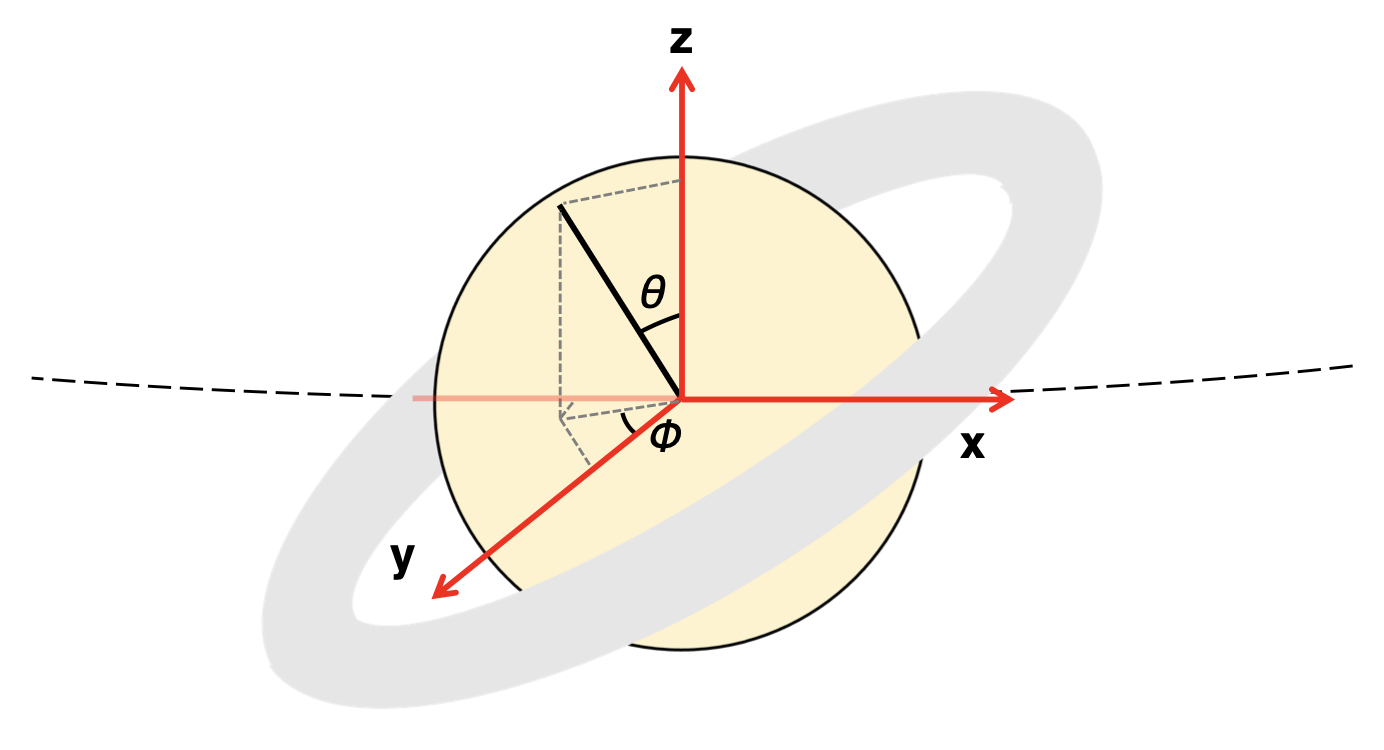
\includegraphics[width=\textwidth]{ring_model_explain.png}
  \caption{our ring model.}
  \label{fig:ring_model_explain}
\end{figure}

\begin{figure}
  \centering
  \includegraphics[width=\textwidth]{0.99_0.0001.png}
  \caption{ringed transit model and ringless transit model.}
  \label{fig:fitting simulation}
\end{figure}

\begin{figure}
  \centering
  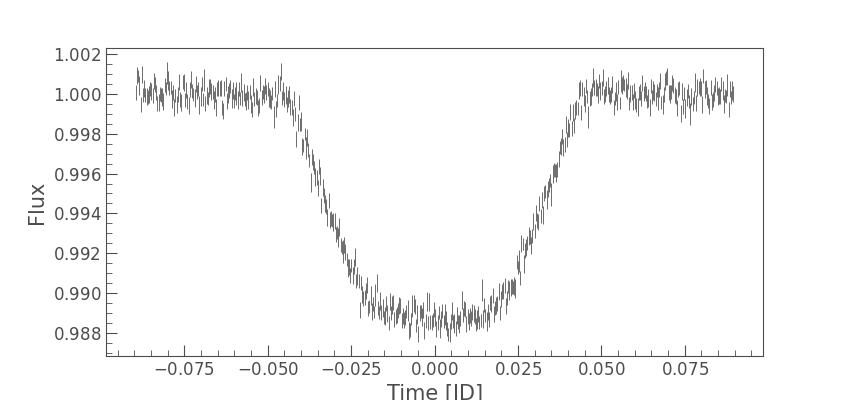
\includegraphics[width=\textwidth]{TOI501.01.png}
  \caption{fail to fit our target.}
  \label{fig: fail fitting}
\end{figure}

\includepdf[scale=0.8]{analysis_flow.pdf}\label{fig:analysis_flow}

\clearpage
\begin{center}
\begin{tabular}{|c|c|c|c|c|}
  \hline
  TOI & depth & sigma & $(\chi^{2}_{\rm{ringless}},\chi^{2}_{\rm{ring}}, N_{\rm{bin}})$ & p \\
  \hline
102.01 & 0.985 & 0.0002 & (687.01, 683.25, 500) & 0.66 \\
105.01 & 0.988 & 0.0004 & (486.34, 484.21, 494) & 0.76 \\
106.01 & 0.992 & 0.0002 & (561.72, 556.40, 500) & 0.41 \\
107.01 & 0.987 & 0.0007 & (1208.48, 1204.49, 500) & 0.86 \\
112.01 & 0.985 & 0.0005 & (506.34, 501.46, 500) & 0.4 \\
114.01 & 0.993 & 0.0002 & (475.68, 472.01, 500) & 0.5 \\
116.01 & 0.983 & 0.0009 & (385.56, 383.69, 498) & 0.71 \\
135.01 & 0.989 & 0.0004 & (718.94, 711.55, 500) & 0.38 \\
159.01 & 0.989 & 0.0006 & (486.20, 485.67, 500) & 1 \\
185.01 & 0.989 & 0.0002 & (572.85, 568.82, 500) & 0.54 \\
195.01 & 0.986 & 0.0005 & (575.85, 573.01, 479) & 0.72 \\
201.01 & 0.993 & 0.0003 &  &  \\
231.01 & 0.976 & 0.0015 & (506.19, 503.61, 499) & 0.69 \\
232.01 & 0.973 & 0.0011 & (488.90, 487.02, 500) & 0.81 \\
391.01 & 0.980 & 0.0011 & (491.72, 490.77, 499) & 0.98 \\
398.01 & 0.981 & 0.0005 & (610.73, 607.31, 500) & 0.65 \\
413.01 & 0.988 & 0.0004 & (472.80, 471.10, 500) & 0.83 \\
418.01 & 0.981 & 0.0009 & (495.53, 494.35, 494) & 0.95 \\
423.01 & 0.983 & 0.0007 & (532.43, 528.97, 500) & 0.58 \\
472.01 & 0.957 & 0.0022 & (483.26, 478.06, 500) & 0.36 \\
495.01 & 0.981 & 0.0004 & (684.75, 681.50, 500) & 0.72 \\
501.01 & 0.987 & 0.0005 & (491.85, 488.72, 500) & 0.59 \\
505.01 & 0.989 & 0.0005 & (484.79, 481.37, 500) & 0.54 \\
621.01 & 0.994 & 0.0003 & (706.57, 701.95, 442) & 0.63 \\
655.01 & 0.978 & 0.0013 & (478.14, 477.11, 500) & 0.96 \\
656.01 & 0.973 & 0.0009 & (457.94, 454.79, 493) & 0.56 \\
675.01 & 0.987 & 0.0005 & (1271.16, 1268.88, 500) & 0.98 \\
758.01 & 0.979 & 0.0009 &  &  \\
780.01 & 0.978 & 0.0011 & (533.78, 530.22, 484) & 0.58 \\
834.01 & 0.986 & 0.0007 & (743.34, 742.16, 500) & 0.99 \\
890.01 & 0.958 & 0.0019 & (1309.41, 1284.26, 476) & 0.2 \\
1019.01 & 0.979 & 0.0009 & (727.47, 724.71, 500) & 0.81 \\
1025.01 & 0.995 & 0.0002 &  &  \\
1085.01 & 0.986 & 0.0004 & (497.97, 494.97, 500) & 0.61 \\
1148.01 & 0.991 & 0.0002 & (939.29, 936.94, 500) & 0.94 \\
1150.01 & 0.993 & 0.0001 & (3922.36, 3826.08, 500) & 0.13 \\
1151.01 & 0.986 & 0.0002 & (1512.77, 1505.61, 500) & 0.72 \\
1161.01 & 0.992 & 0.0004 & (550.11, 547.63, 500) & 0.74 \\
1165.01 & 0.979 & 0.0002 & (457.81, 453.58, 500) & 0.42 \\
1181.01 & 0.993 & 0.0002 & (472.66, 471.70, 500) & 0.97 \\
1186.01 & 0.991 & 0.0003 &  &  \\
1190.01 & 0.992 & 0.0002 & (567.31, 564.68, 500) & 0.73 \\
1236.01 & 0.978 & 0.0009 & (751.34, 747.95, 500) & 0.74 \\
1251.01 & 0.989 & 0.0004 & (455.97, 451.61, 500) & 0.41 \\
1259.01 & 0.971 & 0.0005 & (430.35, 427.28, 500) & 0.53 \\
1265.01 & 0.993 & 0.0003 & (525.80, 524.66, 500) & 0.96 \\
1283.01 & 0.982 & 0.0009 &  &  \\
1295.01 & 0.992 & 0.0003 & (431.09, 429.78, 500) & 0.89 \\
1300.01 & 0.991 & 0.0004 & (557.51, 552.20, 500) & 0.41 \\
1351.01 & 0.985 & 0.0004 & (516.07, 513.11, 500) & 0.63 \\
1431.01 & 0.995 & 0.0002 & (1182.26, 1178.60, 500) & 0.88 \\
1455.01 & 0.982 & 0.0006 &  &  \\
1465.01 & 0.976 & 0.0009 & (372.39, 369.97, 500) & 0.58 \\
1612.01 & 0.990 & 0.0004 & (540.42, 533.63, 500) & 0.3 \\
1651.01 & 0.985 & 0.0005 & (659.50, 651.01, 500) & 0.3 \\
1682.01 & 0.991 & 0.0002 & (794.42, 786.87, 500) & 0.41 \\
1714.01 & 0.987 & 0.0005 & (482.65, 480.76, 500) & 0.8 \\
1725.01 & 0.983 & 0.0005 & (262.48, 261.10, 500) & 0.67 \\
1766.01 & 0.990 & 0.0004 & (705.07, 701.42, 500) & 0.68 \\
1771.01 & 0.985 & 0.0004 & (820.46, 814.98, 500) & 0.56 \\
1864.01 & 0.981 & 0.0008 & (411.24, 410.50, 500) & 0.98 \\
1924.01 & 0.991 & 0.0002 & (1044.06, 1040.41, 500) & 0.84 \\
2014.01 & 0.993 & 0.0003 & (498.13, 496.49, 500) & 0.86 \\
2021.01 & 0.979 & 0.0011 & (338.89, 336.82, 420) & 0.69 \\
2126.01 & 0.975 & 0.0010 & (401.30, 398.23, 500) & 0.5 \\
2131.01 & 0.988 & 0.0004 & (517.04, 509.46, 500) & 0.26 \\
2140.01 & 0.986 & 0.0007 & (462.47, 452.25, 500) & 0.15 \\
2403.01 & 0.987 & 0.0002 & (657.93, 649.78, 500) & 0.31 \\
2547.01 & 0.984 & 0.0008 & (469.34, 466.11, 500) & 0.55 \\
4087.01 & 0.986 & 0.0008 & (498.81, 497.63, 500) & 0.95 \\
4470.01 & 0.974 & 0.0002 & (1375.91, 1369.15, 500) & 0.71 \\
4612.01 & 0.994 & 0.0002 & (665.67, 659.04, 500) & 0.39 \\
5074.01 & 0.990 & 0.0003 & (628.26, 620.99, 500) & 0.33 \\
5096.01 & 0.978 & 0.0010 & (484.57, 480.36, 468) & 0.48 \\
5144.01 & 0.980 & 0.0008 & (484.85, 481.32, 500) & 0.52 \\
5801.01 & 0.965 & 0.0014 & (328.89, 324.60, 356) & 0.42 \\
5821.01 & 0.993 & 0.0003 & (882.96, 882.07, 500) & 1 \\
5823.01 & 0.983 & 0.0008 & (2349.84, 2285.45, 380) & 0.17 \\



\hline
\end{tabular}
\end{center}

%%%%%%%%%%%%%%%%%%%% REFERENCES %%%%%%%%%%%%%%%%%%

% The best way to enter references is to use BibTeX:

\bibliographystyle{mnras}
\bibliography{example} % if your bibtex file is called example.bib

% Alternatively you could enter them by hand, like this:
% This method is tedious and prone to error if you have lots of references
%\begin{thebibliography}{99}
%\bibitem[\protect\citeauthoryear{Author}{2012}]{Author2012}
%Author A.~N., 2013, Journal of Improbable Astronomy, 1, 1
%\bibitem[\protect\citeauthoryear{Others}{2013}]{Others2013}
%Others S., 2012, Journal of Interesting Stuff, 17, 198
%\end{thebibliography}

%%%%%%%%%%%%%%%%%%%%%%%%%%%%%%%%%%%%%%%%%%%%%%%%%%

%%%%%%%%%%%%%%%%% APPENDICES %%%%%%%%%%%%%%%%%%%%%

\appendix

\section{Some extra material}


%%%%%%%%%%%%%%%%%%%%%%%%%%%%%%%%%%%%%%%%%%%%%%%%%%


% Don't change these lines
\bsp	% typesetting comment
\label{lastpage}
\end{document}

% End of mnras_template.tex